For our task of colorising SAR images we require an extensive dataset of paired Sentinel 1 and Sentinel 2 images. Along with the image pairs, we also require additionally metada for text conditioning during the colorisation process. This chapter delves into the extensive process of metadata choices and image acquisition.

\section{Dataset specification}

One of the most crucial information a dataset provides is the metainformation for the items in it. Therefore, we have decided on a set of information that accompanies every image provided with the dataset.

Each image in the dataset has the following common attributes:
\begin{itemize}
    \item \textbf{Coordinates:} Geo-coordinates of the top-left point of the image.
    \item \textbf{Country:} Name of the country where the image was captured.
    \item \textbf{Date-Time:} Date and time when the image was captured.
    \item \textbf{Resolution Scale:} Geospatial resolution of the image.
    \item \textbf{Temperature Region:} Temperature zone of the region in the image.
    \item \textbf{Season:} Season in the specific region at the time the image was captured.
\end{itemize}

Sentinel 1 images have two more attributes to them:
\begin{itemize}
    \item \textbf{Operational Mode:} It is the operational/acquisition mode of the satellite it used to capture the given image.
    \item \textbf{Polarisation:} It is the polarisation with which the image was captured.
\end{itemize}

Sentinel 2 images have one unique attribute:
\begin{itemize}
    \item \textbf{Bands:} Sentinel 2 images come with multiple different information channels called bands, this attribute contains a list of the bands in the image.
\end{itemize}

These were all the metadata associated with the images in the dataset. This information is later leveraged as additional information for text guidance in the colorisation process.

\section{Image acquisition}

Now, that the metadata keys have been decided, we need to select appropriate values for them. Once the values are decided, they can be used to acquire images from the ESA's Copernicus API.

\subsection{Satellite operational mode}

Sen 1 IW

\subsection{Polarization}

VV VH

\subsection{Resolution Scale}

10m

\subsection{Season Classification}

Now, it is needed to classify the season for an image depending on its country and the timestamp from when the image was captured. To do so, we will need seasonal duration data for all countries. This information is not always available for all countries. Also, the seasons are not always the same 4 seasons for all countries, especially given current circumstances with global climate. Hence we need to devise a standardised method to classify seasons for various countries into the four major seasons: \textbf{Winter}, \textbf{Spring}, \textbf{Summer}, and \textbf{Fall}.

To perform this task, we devised an algorithm. It goes as follows:
\begin{enumerate}
    \item Acquire a list of all countries along with a few cities from each country. This is done by using the Simple Maps World Cities dataset\cite{world_cities}. This dataset contains a list of 248 countries along with a few cities from each country and their coordinates.
    \item Retrieve historical weather data (daily average temperature) for a span of a year for every city under each country. This data is retrieved from Open-Meteo\cite{Zippenfenig_Open-Meteo} which provides free API access for various categories of weather data.

    Relevant code snippet can be found in Appendix A. Listing \ref{code:season}.
    \item Average the temperature across all cities for a country to find the daily average temperature of the country over a year.
    \item Find maximum temperature and minimum temperature for each country. This information will be used to calculate time periods for the seasons. It is done in the following way:
    \begin{itemize}
        \item The maximum temperature is considered the peak of summer and the minimum temperature is considered the trough of winter.
        \item The temperatures have an accuracy of 9 significant figures after decimal, so chances of collision (ie., two or more peaks or trough) is almost negligible. Yet, to account for collision, we need to check the hemisphere information.

        If the country is in northern hemisphere, Choose the first peak and trough and vice-versa for southern hemisphere. The reasoning behind this is the general opposite climate in both the hemispheres.
        \item We find the difference between the temperatures, consider it \textit{D}.
        \item Consider \textit{D/4} temperature difference from maximum temperature the onset and end of summer, the same goes for the \textit{D/4} temperature difference from winter. This temperature is called the \textit{transition point}.
        \item Traverse through days towards the past from peak temperature to find a day that has the \textit{transition point} temperature. This is end of spring. Traversing towards future from trough will give us the onset of spring. Similarly in the opposite manner we can fine onset and end of fall.
        \item To find this day, we include a buffer period of 7 days before matching temperature. This is to ensure that a season lasts at least for the duration of a week.
    \end{itemize}
    \item Thus we now have seasonal data for every country.
    \item For contingency, for any country whose data could not be calculated will rely on the classical meteorological season segragation.
\end{enumerate}

This seasonal classification data is later used to map the season metadata value for images.

\subsection{Temperature Region Classification}

Temperature regions are also known as heat zones of the Earth. There are three heat zones, Arctic or Frigid zone, Temperate zone, and Tropical or Torrid Zone. These zones are classified according to latitude.

\begin{itemize}
    \item Tropical Zone: It lies between the Tropic of Cancer ($23.5^\circ$ North) and Tropic of Capricorn ($23.5^\circ$ South). This zone receives the most heat from the sun.
    \item Temperate Zone: In the northern hemisphere, this zone lies between Tropic of Cancer and the Arctic circle ($66.5^\circ$ North). In the southern hemisphere, it lies between Tropic of Capricorn and Antarctic circle ($66.5^\circ$ South).This region is moderately cooler compared to the tropical region.
    \item Arctic Zone: In the northern hemisphere, it is located between the North Pole ($90^\circ$ North) and Arctic circle. In the southern hemisphere, it lies between the South Pole ($90^\circ$ South) and the Antarctic circle. This region is the coldest region of them all.
\end{itemize}

Temperature region data is included in the metadata with the images.

\subsection{Copernicus API}

Copernicus Data Space Ecosystem with a tagline of Europe's eyes on Earth is an open ecosystem that provides free instant access to a wide range of data and services from the Copernicus Sentinel missions\cite{copernicusHome}. It provides data from all Sentinel satellites in various forms.

For Sentinel 1 images we used the "Level 1 Ground Range Detected (GRD)" collection and for Sentinel 2 images we used "Level 3 Monthly Mosaics" collection. The following sections contain an overview of how the copernicus API was used to obtain the images for the dataset.

\subsubsection{Generating coordinates}

Coordinates are generated randomly over the world but are majorly limited to landmass only with a few coastline data. The reason for being majorly landmass is that, the major SAR usefulness comes from it imaging landmass data through clouds. For ocean or water body data, SAR imaging is not used, rather high resolution optical images are used.

After generating random coordinates, they are matched with Natural Earth Land Data\cite{naturalearthland} to ensure the coordinates are from landmass only. Then a few coastline data are taken and verified using Natural Earth Coastline Data\cite{naturalearthcoast}.

The Copernicus service provides a limited number of API calls per month for free users (30,000 calls). To maximize efficiency of API call usage, we decided to obtain images of the maximum size limit offered by Copernicus. The maximum limit is $2500\times2500$ pixels per image. Now, the scale of images need to be 10m.

\begin{align*}
    \text{Hence, ground distance per pixels} &= 10m \\
    \text{Total distance for 2500x image is} &= 10\times2500 \\
    &= 25,000m
\end{align*}

Thus, we need to create square patches with 25 KM distances as the side of the said patch. For this task, we take the randomly generated coordinates and calculate the subsequent latitude and longitude coordinates beginning from that for a consecutive 3 patches. The formulas for approximately converting longitude and latitude into kilometers are as follows:

\begin{itemize}
    \item \textbf{Latitude: } $1^\circ = 110.574$KM
    \item \textbf{Longitude:} $1^\circ = 111.320\times cos(latitude)$ KM
\end{itemize}

Thus, we end up with a list of coordinates for all regions.

\subsubsection{Defining Image Properties}

First we need to do authentication and then, the image properties are set in preparation of the image download. This is where the difference in obtaining Sentinel-1 and Sentinel-2 images appear due to differences in image formats.

We set the image height and width to 2500 pixels each. Following that, the eval script is set. An eval script is a piece of Javascript code which defines how the satellite data shall be processed by Sentinel Hub\cite{evalDoc}. Two different eval scripts are used for Sentinel-1 and Sentinel-2 images due to the different number of bands being used in the images.

The Sentinel-1 eval script is as follows:

\begin{lstlisting}[language=Java]
    //VERSION=3
    function setup() {
        return {
            input: ["VV"],
            output: { bands: 1 }
        };
    }

    function evaluatePixel(sample) {
        return [sample.VV];
    }
\end{lstlisting}

The Sentinel-2 eval script is as follows:

\begin{lstlisting}[language=Java]
    //VERSION=3
    function setup() {
        return {
            input: ["B02", "B03", "B04"],
            output: { bands: 3 }
        };
    }

    function evaluatePixel(sample) {
        return [2.5 * sample.B04/10000, 2.5 * sample.B03/10000, 2.5 * sample.B02/10000];
    }
\end{lstlisting}

From the eval scripts we can infer that Sentinel-1 images have one band, called "VV". It is the polarization of the captured image. "VV" is vertical polarization, i.e.,  vertically transmit and vertically receive. And Sentinel-2 images have 3 bands, namely, B02, B03, B04. The bands are for Blue, Green, and Red channel respectively. The Sentinel-2 images are also preprocessed before download by scaling and normalizing the pixel values. 

Then, bounding box coordinates and time frame for images are sent with the request along with the previously mentioned data.

\subsection{First Manual Inspection}

Once the images are downloaded, the first manual inspection is performed. We check the pair of images to verify that the images contain visible patterns and variations throughout its entirety. Images which had regions of no variation were discarded.

\subsection{Cropping Images}

After the first manual inspection, the images were cropped and divided into multiple smaller images to the decided resolution. The downloaded images have a dimension of $2500\times2500$ pixels. They are divided into 81 $256\times256$ sized images each. This results in a minor loss of information. Figure \ref{fig:cropStep} shows the visualisation of this step.

\begin{figure}[h]
    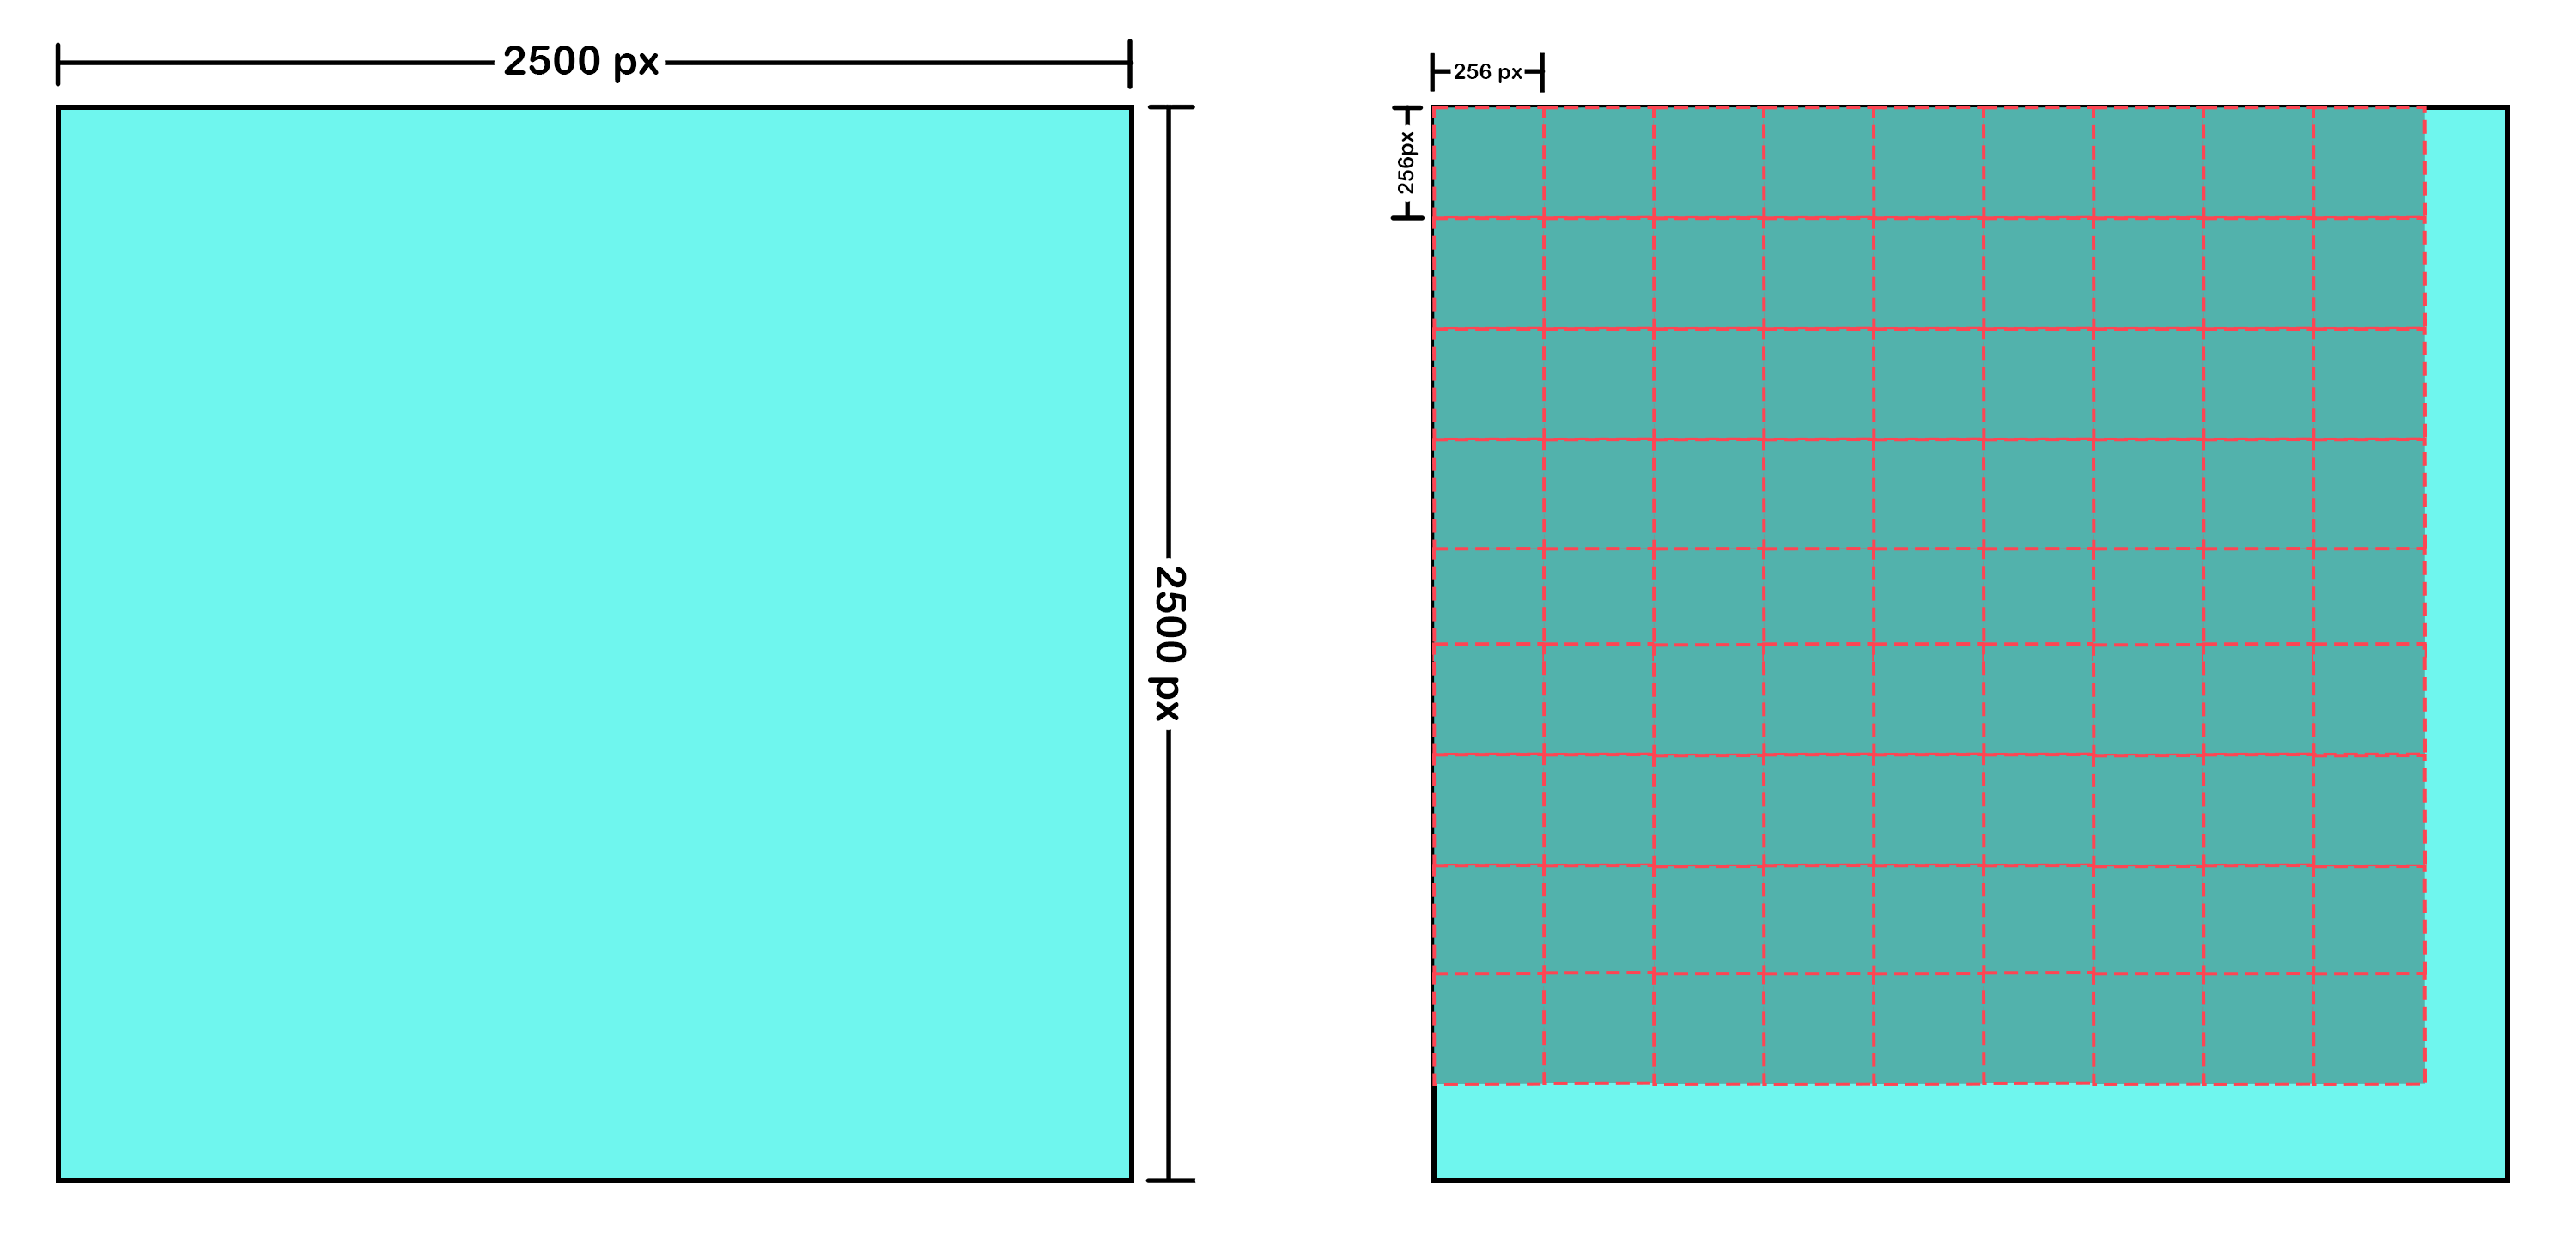
\includegraphics[width=\textwidth]{cropStep.png}
    \caption{Image demonstrating the step of cropping and dividing the large image into smaller images.}
    \label{fig:cropStep}
\end{figure}

\subsection{Second Manual Inspection}

Once the images are cropped and divided into smaller images, one last manual inspection is performed. The purpose of this inspection is the same as the first manual inspection, to verify variations in images. This check is performed to ensure no plain images exist in the dataset.

\subsection{Pre-Processing}

Now, we have arrived at one of the most important steps in dataset preparation. Pre-processing of the images in the dataset. Right from the beginning, there are two issues that remote sensing images face, namely, \textbf{Geometric Distortions due to tilt} and \textbf{Speckle noise}. To fix these issues we tackle them in the following ways:

\subsubsection{Orthorectification}

\subsubsection{Speckle filtering}

\subsection{Organizing and Dataset Structure}

folders